\chapter{Theoretical Background}\label{sec:background}
\section{Simplified Molecular Input Line Entry Specification - SMILES}\label{sec:smiles}
The \ac{smiles} refer to a specific formalism to generate identifiers for chemical compounds that are suited for chemists and computational input. The identifier, in this case, is deduced from a two-dimensional graph of the chemical structure. The result is a series of characters that contain mostly alphanumeric symbols, brackets and some other symbols. The selection of those symbols follows a specific order and a specific set of rules. The set of rules addresses six categories: atoms, bonds, branches, cyclic structures, disconnected structures and aromaticity. Also, \ac{smiles} considers stereochemical information. However, that is not mandatory since the initial approach to \ac{smiles} covers solely two-dimensional information.\cite{Weininger1988}
Atoms are labelled by their element symbol. All elements of a \ac{smiles} string are written in square brackets with the exceptions of the organic subset, i.e. B, C, N, O, P, S, F, Cl, Br, and I. Hydrogen atoms have further specifications. They can either appear implicitly with members of the organic subset. In that case, the remainder of the lowest valence is filled with hydrogen atoms. For example, [C] refers to \ch{CH4}. Explicit notation of hydrogen atoms occurs when they are attached to an element that is not part of the organic subset. Given a metal M, the nomenclature of four hydrogen atoms attached to that metal is [MH4]. Hydrogen can also be mentioned on its own in brackets [H], e.g. in its molecular form \ch{H2}. Charges are represented with a plus or minus with their respective count inside a bracket.\cite{Weininger1988}
Bonds within the \ac{smiles} nomenclature are omitted if they are either aromatic or single covalent bonds. Double bonds are represented with '\ch{=}', and triple bonds are represented by '\#'. Ionic bonds are not explicitly denoted by the \ac{smiles} algorithm. An ion pair is written as two disconnected structures with formal charges to them. Tautomeric bonds are not explicitly denoted either. One of the possible structures is translated into the \ac{smiles} string, be it the enol or keto variation.\cite{Weininger1988}\\
Branches are depcited in parenthesis. 5-Methyl-4-(2-methylpropyl)-4-(propan-2-yl)hept-1-ene is an example of nested branching using nested parenthesis. The name of the structure is according to the convention of \ac{iupac}\cite{2014a}. The structure and \ac{smiles} is shown in \fref{fig:branching}.
\begin{figure}[H]
	\centering
	\includegraphics[width=0.9\textwidth]{figures/branch.pdf}
	\caption[Demonstration of a Branching Structure with SMILES]{On the left, side a model compound is shown as an example of nested branching in \ac{smiles}. On the right, the \ac{iupac} name and its \ac{smiles} string are shown. The \ac{smiles} string features parenthesis that imply branching and nested branching.\cite{Weininger1988}}
	\label{fig:branching}
\end{figure}\noindent
Cyclic structures are written linearly by breaking a single or aromatic bond within the cycles. Next, the broken bonds are arbitrarily labelled by writing the formerly connecting elements right in front of a number assigned to the broken bond. An illustrating example is shown in \fref{fig:cycle}.
\begin{figure}[H]
	\centering
	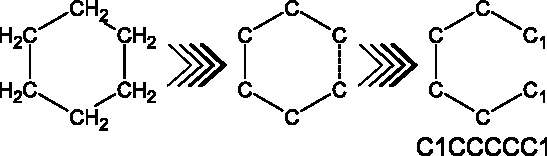
\includegraphics[width=0.5\textwidth]{figures/cycle.pdf}
	\caption[SMILES string of a Cyclic Structure]{Cyclohexane as an example for a cyclic structure. First, the explicit hydrogens are exchanged for implicit ones, and the ring is linearized by conceptually breaking a bond implied by the dashed line. The carbons connected by the dashed line are being labelled, and the resulting \ac{smiles} string is shown below the right-hand structure.\cite{Weininger1988}}
	\label{fig:cycle}
\end{figure}\noindent
A single atom can be part of multiple rings which is then accounted for by using two or three single digits in sequence. However, for structures with more than ten rings, double digits are separated with a prefacing per cent sign. Also, a single digit can be reused for multiple broken bonds without creating ambiguity. A \ac{smiles} string is read from left to right, and a ring closes on the first repetition of a respective digit. Cubane is an example that has multiple rings. In \fref{fig:cycles} the generation of a \ac{smiles} string is shown with the usage of the digit '1'. \cite{Weininger1988}
\begin{figure}[H]
	\centering
	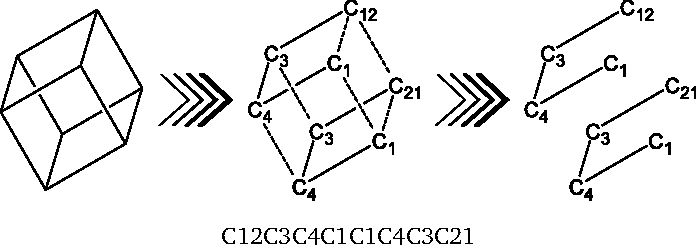
\includegraphics[width=0.7\textwidth]{figures/cubane.pdf}
	\caption[SMILES String that Resembles Multiple Cycles within the Same Molecule]{Cubane as an example of a structure that has multiple cycles. On the left, the structure is shown without explicit hydrogen atoms. In the middle picture, the bonds that are artificially broken to linearize the molecule for the \ac{smiles} string are shown in dashes. On the very right, the skeleton structure resembles the \ac{smiles} string, that is written below the molecular representations.\cite{Weininger1988}}
	\label{fig:cycles}
\end{figure}\noindent
A \ac{smiles} string is read from left to right, and a ring closes on the first repetition of a respective digit. Disconnected structures are written as individual \ac{smiles} strings separated by a comma. \cite{Weininger1988}\\
Aromaticity is denoted by writing the atoms that are part of an aromatic cycle in lower case letters. Aromaticity is detected by applying an extended definition of H\"uckel's rule. Another noteworthy convention is the treatment of aromatic nitrogen atoms. A nitrogen atom that is embraced by two aromatic bonds has no valency left per default. However, for aromatic nitrogen that is connected to a hydrogen atom, the hydrogen atom is specified as shown in \fref{fig:nitrogen}.\cite{Weininger1988}
\begin{figure}[H]
	\centering
	\includegraphics[width=0.9\textwidth]{figures/aromaticnitrogen.pdf}
	\caption[Specifications for Aromatic Nitrogen within the \ac{smiles} algorithm]{Different instances of aromatic nitrogen. Notice that the \ac{smiles} string of pyrrole contains an additional hydrogen atom that preceded the aromatic nitrogen. The aromaticity of an atom is denoted by writing it in lower case letters.\cite{Weininger1988}}
	\label{fig:nitrogen}
\end{figure}\noindent
Furthermore, the \ac{smiles} algorithm introduces a convention for labelling double bond configurations and chirality. The double bond configuration is indicated by placing '/' or '\textbackslash' between the atom constituting the double bond and their subsequent bonding partners. The indicators can be understood as a single bond type that gives information about their relative orientation. An example for (Z)-1,2-difluoroethene and (E)-1,2-difluoroethene is given in \fref{fig:doublebond}.\cite{smilesmanual}
\begin{figure}[H]
	\centering
	\includegraphics[width=0.7\textwidth]{figures/doublebond.pdf}
	\caption[Example of Double Bond Configuration in \ac{smiles} Notation]{Example of double bond configuration in \ac{smiles} notation. On the left (Z)-1,2-difluoroethene is shown and on the right is (E)-1,2-difluoroethene with their \ac{smiles} notation. Both notations shown for each structure are valid.\cite{smilesmanual}}
	\label{fig:doublebond}
\end{figure}\noindent
Chirality is assigned to chiral tetrahedral centres and any other chiral centre, e.g. allene-like or square planar centres. Herein, the \ac{smiles} notation is explained in the context of tetrahedral chirality centres, which is the most straightforward instance of chirality in organic chemistry. A chiral centre can not be the terminal node in a molecular representation since a terminal node is either only connected to hydrogen atoms if any at all. With that in mind, the convention for tetrahedral chirality is most easily explained by investigating an example which is (1S)-1-chloro-1-fluoroethan-1-amine which can be seen in \fref{fig:enantio}. The whole molecule is viewed along the CC-bond. Necessarily, the \ac{smiles} string contains the central C-atom's binding partners in a specific order. This sequence can either correspond to the clockwise or anticlockwise binding partners' order when the molecule is viewed along the CC axis. Should the order be anticlockwise, an '@' is inserted after the central C-atom in brackets. The '@' is a visual mnemonic since it depicts an anticlockwise rotation around the central circle. For a clockwise order, '@@' is used instead of a single '@'.
\begin{figure}[H]
	\centering
	\includegraphics[width=0.8\textwidth]{figures/tetrachiral.pdf}
	\caption[Example of Enantiomere \ac{smiles} Strings]{Example of enantiomer \ac{smiles} strings.\cite{smilesmanual} Both molecules are pictures in the same way. Above each depiction is the name of the chemical formula followed by a schematic. The eye indicates the point of view along the CC axis. The resulting view of the structure is shown on the right of each subfigure. Written below are two equally adequate \ac{smiles} strings for each structure.}
	\label{fig:enantio}	
\end{figure}\noindent
%
%
\section{Canonical SMILES}\label{sec:cansmiles}
In general, \ac{smiles} strings do not claim to be unique identifiers. There are many equivalent options to generate a \ac{smiles} string for a given structure. Nowadays, computational biochemical research accesses structures from many different sources and databases, making the requirement of a unique identifier evident. The \ac{smiles} notation was developed with this objective in mind. So-called canonical \ac{smiles} strings fulfil this objective. They are based on the same set of rules described in \fref{sec:smiles}. The algorithm can be partitioned into two parts: the CANON part and the GENES part. The CANON part labels the atoms of the molecular structure canonically, i.e. a unique way based on the structural topology. The GENES part generates the unique \ac{smiles} from the aforementioned rule set (see \fref{sec:smiles}) and the canonical labelling.\cite{Weininger1989}\\
For finding a unique way of labelling atoms in a molecule, invariant structural properties are necessary. Thus, five properties are considered atomic invariants. Those would be (1) the number of connections, (2) the number of non-hydrogen bonds, (3) the atomic number, (4) the sign of the charge and (5) the number of attached hydrogens. They are called 'invariant' because they are invariant to atomic order changes within a structural notation, and they are exchangeable as long as this principle is not violated. The numbers in the parenthesis in front of each property correspond to a pre-defined prioritization.
In summary, the atomic invariants assign five integers to every atom in a molecule. The so-called individual invariant can be obtained by simply combining these integers in order of their prioritization. Given the methyl carbon of 2-(acetyloxy)benzoic acid in \fref{fig:canonicallabelling} with the individual invariant 110603. From this individual invariant, it can be concluded that this atom has 1 connection, 1 bond to a non-hydrogen neighbour, an atomic number of 06, 0 charge and 3 attached hydrogen atoms.
Other atomic properties like isotopic mass and local chirality can be added if these six properties are not sufficient to discriminate all distinguishable nodes from each other. It is noteworthy that some nodes are symmetric and require a tie-breaking function for absolute uniqueness (see next paragraph).\cite{Weininger1989}\\
After assigning every atom an individual variant, those are compared among all constituting atoms and are ranked by magnitude. The final atom labels depend on the topology, as well. Therefore, the nodes (atoms) rank is extended by its corresponding prime (for 1, 2, 3, the corresponding primes are 2, 3, 5). The so-called new invariant is obtained by multiplying the corresponding primes of all neighbours for every atom. Afterwards, ranks are assigned again, based on their current rank and new invariant. The procedure is repeated iteratively until the combined invariant is not changing anymore. Should there be constitutionally symmetric nodes present in the molecular graph, it becomes necessary to break ties since the symmetric groups make it impossible to find a ranking that offers a completely ordered set of nodes necessary for finding a canonical \ac{smiles} representation. For tie-breaking, all ranks are doubled, and the first instance of an asymmetric node is decremented by one. The resulting node ranking is considered a new invariant set that goes through the aforementioned iterative process of corresponding prime multiplication until it is no longer changing. After every rank is of the combined invariant is unique and not changing upon further iteration, the uniquely ordered ranking has been accomplished.\cite{Weininger1989} The canonical labelling process for 2-(acetyloxy)benzoic acid is shown in \fref{fig:canonicallabelling}.
\begin{figure}[H]
	\centering
	\includegraphics[width=0.9\textwidth]{figures/canonical_labelling.pdf}
	\caption[Canonical Labelling with 2-(Acetyloxy)Benzoic Acid]{Canonical labelling with 2-(acetyloxy)benzoic acid. Every row corresponds to consecutive iterations of the CANON algorithm. The blackboard bold $\mathbb{P}$ denotes finding corresponding primes. The greek letter $\Pi$ denotes taking the prime products of all atoms, and the hashtag denotes atoms' ranking. Bold numbers denote ranks that reached invariance.}
	\label{fig:canonicallabelling}	
\end{figure}\noindent
THE GENES part of the algorithm can utilize the uniquely ordered ranking to chose the start node and prioritize at branching points, etc. As an entry point for the generation of canonical \ac{smiles}, the node with the lowest ranking is chosen. Branching decisions are made in the same fashion, i.e. the branching option with the lowest rank is chosen and followed until a dead end has been reached. A special rule applies when branching into a ring with a double or triple bond. To avoid opening the ring at any multi-bond, the algorithm will always branch towards the multi-bond. Also, the ring-opening digits must be in the order of ring-opening nodes.\\
Conclusively, a unique \ac{smiles} string can be assigned by first generating a unique invariant rank for every node that incorporates invariant atomic properties and topological information and then using these ranks as decision indicators for branching and cycles.\cite{Weininger1989}
%
%
\section{Extended-Connectivity Fingerprints}\label{sec:extendedconnectivityfingerprints}
The \ac{ecfp} is a structural fingerprint that was developed to capture molecular features relevant for molecular activity.\cite{Rogers2010} \acp{ecfp} are also commonly referred to as Morgan-fingerprints since their development is partially based on the Morgan-algorithm which pursues rigorous canonicalisation similar to the CANON algorithm in \fref{sec:cansmiles}.\cite{Morgan1965} 
The procedure of the algorithm can be distinguished into two parts: the initialization (or zeroeth iteration) and the iteration process.\\
For initialization, all atoms in the molecule are given an identifier that is computed from six atomic invariants, similar to the ones in \fref{sec:cansmiles} canonical \ac{smiles} algorithm (number of connections, number of bonds, atomic number, atomic mass, atomic charge, number of attached hydrogens).\cite{smilesmanual} However, a seventh invariant is taken into account: whether the atom is part of at least one ring structure. A hashing algorithm maps the atomic invariants to a 32-bit integer. Any functional hashing algorithm that reproducibly maps the input onto a 32-bit integer is a sensible choice since the only requirement is that a variant is uniquely mapped to the same 32-bit integer every time it is hashed. The 32-bit integer is also referred to as the core identifier. Within the initialization step, it corresponds to a substructure that contains information about one atom and its bonds and is appended to a list called \acl{eset}. After completion of the algorithm, the \acl{eset} is equal to the fingerprint.\cite{Rogers2010} Therefore, the result of the initialization are a set of core identifiers [$c^{(0)}_0,c^{(0)}_1,c^{(0)}_2,...,c^{(0)}_n$]. The core identifier for atom 1 of the initialization (zeroeth iteration) would be $c^{(0)}_1$.\\
After the initialization the first iteration starts by randomly picking an atom, let that be atom 4. Next, the iteration number (1) and the core identifier, $c^{(0)}_4$, are appended to a temporary list. Afterwards, the neighbouring core identifiers are appended to the temporary list together with their respective bond order. $b_{4j}$ denotes the bond order between atom 4 and its neighbour, $j$. The bond order can either be 1, 2, 3 or 4 for aromatic bonds. Let the resulting temporary list have the following format $[1,c^{(0)}_4,b_{34},c^{(0)}_3,b_{45},c^{(0)}_5,b_{46},c^{(0)}_6]$. In this example the temporary list comprises eight entries which are inputted into a hashing function that returns a 32-bit integer. This integer is the core identifier of atom 4 for, $c^{(1)}_4$. Once this process is completed for every atom, all core identifiers are updated to the new core identifier simultaneously and are appended to the \acl{eset}. The temporary lists are being discarded. After iteration 1, the \acl{eset} comprises of the elements $[c^{(0)}_0,...,c^{(0)}_n,c^{(1)}_0,...,c^{(1)}_n]$.\cite{Rogers2010}\\
The second iteration is conducted in the same way as the first iteration. However, the core identifier of $j$ of the first iteration contains information about its surrounding cores and their bonds. Therefore, information from up to two bonds is incorporated into the second iteration's core identifiers, $c^{(2)}_j$. Thus, from iteration to iteration, the core identifiers can be understood as the core atom within a larger and larger structural neighbourhood. $c^{(0)}_j$ is a 32-bit integer that encodes the atom $j$ and its adjacent bonds. $c^{(1)}_j$ is a 32-bit integer that encodes atom $j$, its neighbouring atoms within one bond length, their bond orders and their adjacent bonds, and so on.\cite{Rogers2010}\\
After the specified number of iterations is completed, duplicate 32-bit integers are removed from the \acl{eset} since they encode for the same subtructure. Butyramide is shown in \fref{fig:butyramideecfp} as a conceptual example of fingerprint generation.\cite{Rogers2010}
\begin{figure}[H]
	\centering
	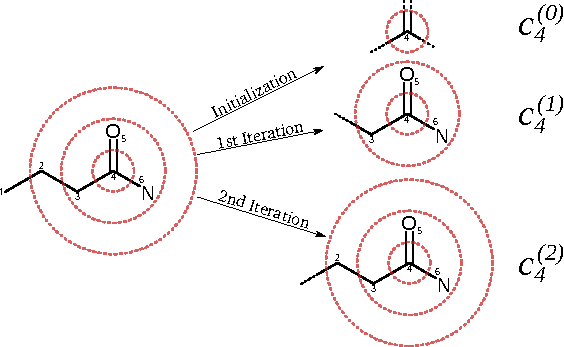
\includegraphics[width=0.6\textwidth]{figures/butyramide_ecfp.pdf}
	\caption[Fingerprint Iterations with Substructures for One Atom]{Fingerprint iterations with substructures for one atom. Atom 4 of butyramide iterated, denoted by the red circles. The smallest circle denotes initialization of atom 4, resulting in $c^{(0)}_4$ only containing information about the core atom and adjacent bonds. The first iteration is denoted by the intermediate circle and results in $c^{(1)}_4$. The second iteration is denoted by the outer circle and results in $c^{(2)}_4$.}
	\label{fig:butyramideecfp}
\end{figure}
So far \acl{eset} contains 32-bit identifier. A substructure could be encoded by the integer, e.g. 1559650422, which would correspond to an "on" bit within a bit set of $2^{32}$ bits. Since a hash space of $2^{32}$ is quite vast, the 32-bit integers are usually mapped onto a vector of 1024 (or 2048) bits by yet another hashing algorithm. Even though the bits in the new 1024-bit-vector cannot be directly decoded into molecular substructures, the identifiers and substructure pairs can be saved and subsequently accessed. In summary, \acp{ecfp} are generated by hashing atomic invariants into identifiers, which are then updated a specified number of times with information of their immediate surroundings. Eventually, the core identifiers are hashed into a bit-vector (usually 1024 or 2048 bits) that indicates present substructures by "on" bits (1) and missing ones by "off" bits (0). The procedure is visualized in \fref{fig:ecfpprocess}.
\begin{figure}[H]
	\centering
	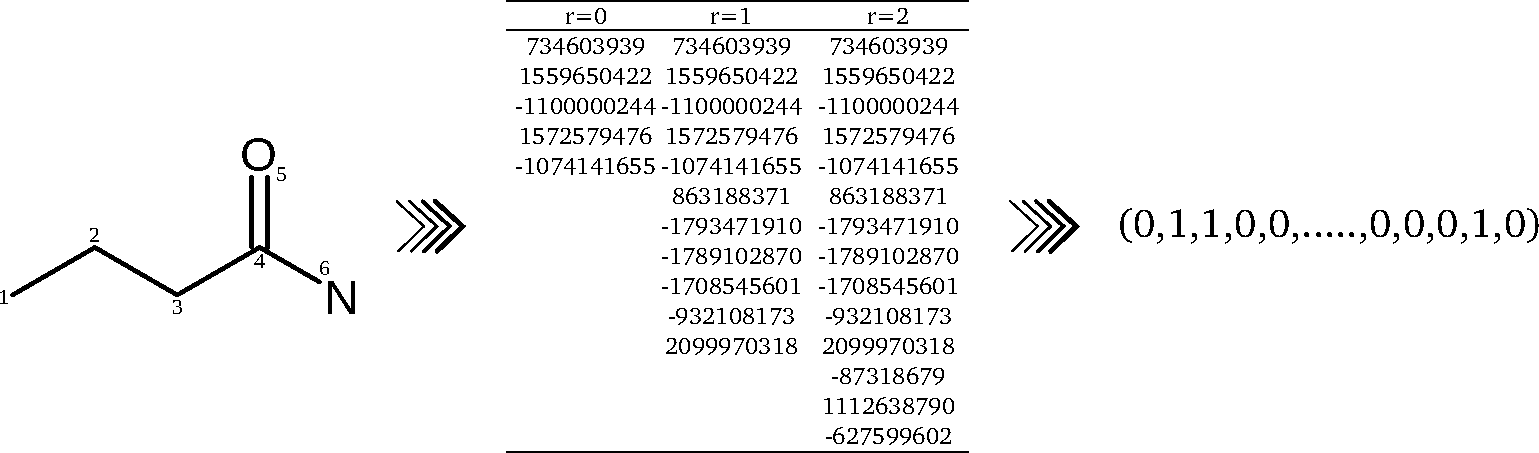
\includegraphics[width=0.8\textwidth]{figures/ecfp_process.pdf}
	\caption[Visualization of \ac{ecfp} Generation]{Butyramide as an example of \ac{ecfp} generation. Starting from the structure, the identifiers are generated for radius 0, 1, and 2 and appended to the \acl{eset}. From the identifiers with radius 2, a bit vector of a certain length is obtained.}
	\label{fig:ecfpprocess}
\end{figure}
\section{Cell-Painting Assay}\label{sec:cpassay}
Cell-Painting (CP) refers to a high-content-screening method that generates cellular image data from high-throughput fluorescence microscopy experiments. A \ac{cp} assay consists of several consecutive steps which result in tabulated raw image data. These steps consist of cell culture, treatment, staining and fixation, automated image acquisition and feature extraction.\cite{Bray2017}\\
This project uses \ac{cp} data generated by the Broad Institute\cite{Bray2017}. U-2 OS cells were used as the target organism in the cell painting assay reported by Bray \textit{et al}.\cite{Bray2017} 1500-2000 cells were seeded into every well of multiple 384-well clear bottom plates and incubated at \SI{37}{\degreeCelsius} for 24 hours.\cite{Wawer2014}\\
Then, compounds were added to the well in quadruplicates of varying concentrations. In total, 30409 different compounds were added and incubated for 48 hours. The compounds used can be categorized as small molecules and were either taken from the \ac{mlsmr}, the known bioactive compounds database of the Broad Institute, the \ac{mlp} or compounds derived from diversity-oriented synthesis. Antibodies, enzymes and other biotherapeutics were not used in this bioassay.\cite{Bray2017}\\
In total, six different fluorescent reagents were used to stain five different cell-organelles. Only two of the reagents were applied to the living cell culture; the remaining four were applied after the cells' fixation. A combination of two reagents was used to stain the F-actin cytoskeleton, plasma membrane and Golgi apparatus. Another reagent is used to stain the nucleoli and the cytoplasmatic \ac{rna}. Additionally, individual reagents are used to stain the \ac{er}, the nucleus and the mitochondria, respectively. The six reagents are listed in \fref{tab:dyes}) with the cell organelles, they respond to and the catalogue number.
\begin{figure}[H]
	\centering
	\includegraphics[width=0.8\textwidth]{figures/cell_figure.pdf}
	\caption[Concept of 5-Channel Imaging]{Concept of 5-channel imaging. The live cell is stained with fluorophors and the imaged in 5 different channels. Each highlighting different compartments in the cell. The highlighted compartments of each channel are opaque and light emission is implied by sparkles.}
	\label{fig:cellfigure}
\end{figure}
\begin{table}[H]
	\begin{center}
		\caption[List of Fluorescents Dyes]{The fluorescent dyes used in the \ac{cp} assay are listed here. The list contains the names of the fluorophours, the cell organelle(s) that they are targeting and the catalogue number that refers to the Invitrogen catalogue.\cite{Wawer2014} The maxima of the excitation and emission wavelengths of the fluorophors are shown in nanometer.}
		\label{tab:dyes}
		\begin{tabularx}{\textwidth}{XXlll}
			\toprule
			Fluorescent reagents & Cell Organelle &  $\hat{\lambda}_{ex}\SI{}{\per\nano\meter}$ & $\hat{\lambda}_{em}\SI{}{\per\nano\meter}$ & Invitrogen\\
			
			\midrule
			
			Mitotracker Deep Red & Mitochondria &644 & 665& M22426\\
			
			Wheat Germ Agglutinin, Alexa Fluor 594& F-actin cytoskeleton, plasma membrane, Golgi & 589 & 615 & W11262\\
			
			Concanavalin A.  Alexa Fluor 488 & ER & 495 & 519 &  C11252\\
			
			Phalloidin, Alexa Fluor 594 & F-actin cytoskeleton, plasma membrane, Golgi& 581 & 609 & A12381\\
			
			Hoechst 33342 & Nucleus & 350 & 461 & H3570\\
			
			SYTO 14 green-fluorescent nucleic acid stain & Cytoplasmatic \ac{rna}, Nucleoli & 521 & 547 & S7576\\
			\bottomrule
		\end{tabularx}
	\end{center}
\end{table}\noindent
After the compound treatment, a staining solution of Mitotracker and \ac{wga} was added and incubated for \SI{30}{\minute} at \SI{37}{\degreeCelsius}. Afterwards, cells were fixed using paraformaldehyde. Afterwards, staining solutions containing Phalloidin, Hoechst 33342, SYTO 14 and Concanavalin were applied to the cell containing wells and incubated for \SI{30}{\minute}. Finally, the plates were thermally sealed and stored at \SI{4}{\degreeCelsius}.\cite{Bray2016,Wawer2014}\\
In the next step, images were generated via automated fluorescence microscopy. Five fluorescence channels were used, which scan the plates for different wavelengths emitted by the fluorophors tagging specific cell organelles. The channels are labelled \ac{dna}, \ac{rna}, AGP (F-actin cytoskeleton, Golgi and plasma membrane), Mito (mitochondria) and ER (Endoplasmatic Reticulum).\cite{Bray2017}\\
After the automatic image acquisition was completed, the so-called CellProfiler\cite{Carpenter2006,Kamentsky2011} software generated numerical features from these images. CellProfiler has its standard pipeline to generate cellular features from fluorescence images. The concepts of this pipeline are visualized in \fref{fig:cellprofiler}. First, the images were aligned, cropped, and an illumination correction is applied, followed by the cell identification step. CellProfiler first identifies nuclei by searching for bright, well-dispersed and non-confluent so-called primary objects. Another important step in this recognition is to identify clumped primary objects, then find their dividing lines and remove them or merge them depending on their measurements.\cite{Carpenter2006} Taking the nuclei as a starting point, the secondary objects, like cell edges, the cytoplasm and nuclear membrane, are identified next. After the cells have been identified, CellProfiler conducts different measurements to calculate various features related to cellular compartments and organelles. These features include the area, shape, texture and other more complex features.\cite{Carpenter2006} The dataset used in this work comprises 1768 features that have a variance greater than 0. Features that remain constant for every compound do not contain any information relevant to this work and are discarded. After the feature extraction via CellProfiler, the finalized data set is called raw image data. 
\begin{figure}[H]
	\centering
	\includegraphics[width=0.8\textwidth]{figures/cellprofiler.png}
	\caption[CellProfiler Workflow]{Conceptual visualization of the CellProfiler workflow. The first image shows fluorescent microscopy images of human cells. These are cropped and rotated to yield a better view of the cells.\cite{Moffat2006}\cite{cellprofiler2021} In the second step, the illumination correction function is applied to a generic image.\cite{cellprofiler2021} In the last step (Object Recognition), the identification of stained nuclei and membranes of human pluripotent stem cells are shown as an example.\cite{McQuin2018} The obtained images were slightly modified.}
	\label{fig:cellprofiler}
\end{figure}\noindent
%
%
\section{Raw Image Data}\label{sec:rid}
CellProfiler extracts numerical features from cellular images. The resulting raw image data is a huge spreadsheet whose columns contain the features, and the rows correspond to wells from which the original images were taken. Additionally, the rows are identified by the compounds used to treat the respective wells, exempt control wells treated with \ac{dmso} only. Every compound is measured in quadruplicates as a minimum. Also, some are measured in octuplicates as well as in different concentrations. There are at least four rows corresponding to four wells in the raw image data spreadsheet for every compound. Compounds whose features have been extracted for only one concentration are referred to as \acl{scc}s and the compounds that appear in multiple concentrations are called multi-concentration-compounds.\\
The spread sheet does not only contain numerical features extracted from CellProfiler but so-called metadata, too. Metadata refers to methodological information relevant for the experimental procedure. Hence, compound concentration, plate number, plate map number and other information are being categorized as metadata. Also, the information whether the row corresponds to a treated or control well, is stored within the first \num{17} columns before the listing of CellProfiler features from column \num{18} to \num{1801}. From these 17 only five are important for the suceeding steps. Among plate, location, role and concentration these columns contain further information about the molecular structure of the respective compound as a \ac{smiles} string (see \fref{sec:smiles}). In \fref{tab:metaheader} the column header names are listed together with a brief description. The names in \fref{tab:metaheader} correspond to the ones from the original raw image data file.\cite{Bray2017}
\begin{table}[H]
	\begin{center}
		\caption[Important Metadata Columns]{Below, the names of the most important metadata column headers are listed verbatim from the source file. For every column header, a description is supplied.}
		\label{tab:metaheader}
		\begin{tabular}{lp{8cm}}
			\toprule
			Column Name & Description\\			
			\midrule
			\texttt{Metadata\_Plate} & Contains the plate number of respective well \\
			\texttt{Metadata\_ASSAY\_WELL\_ROLE}& States if the well was treated with a compound or just with \ac{dmso}\\
			\texttt{CPD\_SMILES}& Contains the compound as a \ac{smiles} string\\
			\texttt{Metadata\_mmoles\_per\_liter}& States the compound concentration for treated samples\\
			\texttt{Metadata\_broad\_sample}& Identifier assigned by Broad Institute that varies inconsistently either with compound, concentration or plate number\\
			\bottomrule
		\end{tabular}
	\end{center}
\end{table}\noindent
%
%
\section{PubChem-Assay}\label{sec:pubchem}
Within the subject of \ac{ml}, targets or labels are referred to as features of interest. An \ac{ml} algorithm attempts to predict targets from a given input similar to a function that calculates $y$ from a given $x$. Labelling cats and dogs images is a vivid example where the label would either be 'cat' or 'dog'. The inputs would be the individual pixels of an image or their numerical color values, to be precise. The same principle can be applied to bio- and chemoinformatics. Typical targets in this scientific area are 'active' and 'inactive' for a certain bioassay. Nevertheless, annotated data that that can be used for labelling is scarce.\\
The database that supplies the targets for this project is the \acl{p} database.\cite{Kim2015} The PubChem database contains information about chemical compounds and their bioactivities found in various assays. The bioassays in \acl{p} are assigned a unique \ac{aid} and possess a data page featuring descriptive information and the corresponding readout. The descriptive part contains, among others, information like the name and theoretical background, experiment procedure, data source and a readout explanation.\cite{Wang2009}\\
In general, the depositor of a bioassay can provide as many detailed results as necessary.\cite{Wang2011} However, \acl{p} requires the depositor to submit a summary result for each chemical sample. This summary result constitutes the numerical 'bioactivity score' and the categorical 'bioactivity outcome'. The bioactivity outcome can assume five mutually exclusive values: 'chemical probe', 'active', 'inactive', 'unspecified' and 'inconclusive'. The rationale behind the bioactivity outcome is usually provided in the assay comment section to enable a detailed interpretation of the users' results.\cite{Wang2009} In the following the bioassay 720532 is described in detail as an example.\\
%
\subsubsection{AID 720532}
Kolokoltsov \textit{et al.}.\cite{Kolokoltsov2007} could prove that virus cell-entry strongly depends on the host-cell mediators. Mediator for cell-entry can be Signalling factors, membrane attachment factors and endosomal and lysosomal factors.\cite{HofmannWinkler2012} By targeting the host-cell mediators, the emergence of drug-resistant virus mutants is less likely since the cellular mutation rates are up to 6 orders of magnitude smaller compared to viruses.\cite{Kolokoltsov2009} The bioassay AID 720532 is an assay that targets cell-entry of the Marburg virus. Non-pathogenic \ac{vsv} with the envelope glycoproteins of the Marburg virus were used as a pseudovirus referred to as VSV-MARV. The pseudovirus contains a Photinus luciferase reporter gene within its genome. Therefore, cell-entry is detected by changes in luminescence. The assay uses HEK293 cells in 1536-well plates. After applying compounds to the respective wells, the plate is incubated. Next, VSV-MARV is applied inf sub-saturating amounts. Luciferase signals reflect the virus titer able to infect the cells for the different compounds.\cite{AID720532}\cite{Kim2020} During a similar screening against Ebola virus entry (same family as Marburg virus), many signalling pathways relevant to cancer, gene regulation and cell cycle control were found relevant in preventing cell-entry.\cite{Kolokoltsov2009}
%
%\subsubsection{AID 651635}
%The expansion of a polyglutamine domain of Ataxin-2  due to a mutation in the \ac{atxn} causes a neurodegenerative disease called \ac{sca2}.\cite{Pulst1996} The objective of bioassay AID 651635 is to find small molecules that inhibit \ac{atxn} expression. For this purpose, SH-SY5Y cells with a ataxin-2-firefly-luciferase transgene are transferred into a 1536-well plate, then treated with compounds and Gly-Phe-7-amino-4-trifluoromethyl coumarin to access cell-viability. Eventually, the luminescence is measured to infer the expression of the ataxin-2-firefly-luciferase transgene.\cite{AID651635} The cell line SH-SY5Y is a neuroblastoma cell line obtained from a human bone marrow biopsy.\cite{Biedler1973}
%
%
\section{SMOTE - Synthetic Minority Oversampling Technique}\label{sec:smote}
\ac{smote} can be used to overcome problems associated with imbalanced data sets. The method uses the given data as input and creates synthetic samples from that data. The process is most easily described for a two-dimensional data set. For every point in that data set, the $k$ nearest neighbours are found. New data points are then generated on the connecting lines in between the central point and its neighbours. The total number of new data points generated between the central point and its surrounding neighbours depends on the sampling strategy, i.e. how many data points the total semi-synthetic data set is supposed to have. The distance at which the synthetic points are inserted is chosen at random.\cite{Chawla2002} For a strong label imbalance, the \ac{ml} algorithm performs well, even if it only classifies one label sufficiently. By generating data points that are presumably representative of the minority class, the \ac{ml} algorithm has to shift its focus towards the minority class to achieve better performance.
\begin{figure}[H]
	\centering
	\includegraphics[width=0.7\textwidth]{figures/smote.pdf}
	\caption[SMOTE Applied to a 2D Data Set]{SMOTE applied to a 2D data set. The minority class (orange) is oversampled and the majority class (blue) is undersampled.}
	\label{fig:smoteexample}
\end{figure}\noindent
%
%
\section{Random Forests}\label{sec:randomforestbackground}
In \ac{ml} classification denotes a (mathematical) rule that produces a label $y$ from a set of input features $X$. One way of classification utilizes a decision tree. A decision tree is a common mathematical tool in stochastics, closely related to the probability tree. In \ac{ml}, the nodes are used as entry points for data to be classified, and the paths after each node are called branches. The final nodes at which the classification process ends are called leaves. The decision tree splits the complete data set, $D$, into subsets, $D_{l}$ and $D_\text{r}$, funnelling them to the left or right branch starting at the root node. The information given by the feature, $f$, guides the splitting of the dataset at each node. Moving further down the branches, the subsets are split into smaller and smaller subsets until they reach the leaves. The leaves correspond to labels present in the data. A leaf assigns its label to every sample of a subset that arrives at the said leaf. A certain numerical rule, the splitting condition, defines how to split the data set, and each node splits the entering data set based on one certain feature. However, since the decision tree is sequential, the information from earlier nodes is always part of the decision process. Therefore, the final decision for the label at the leaves incorporates multidimensional data in a quite simple fashion. A decision tree can be visualized in the context of its data since it applies geometrical decision boundaries (see \fref{fig:decisiontreegraph}).\cite{Forsyth2019}
\begin{figure}[H]
	\centering
	\begin{subfigure}[c]{0.45\textwidth}
		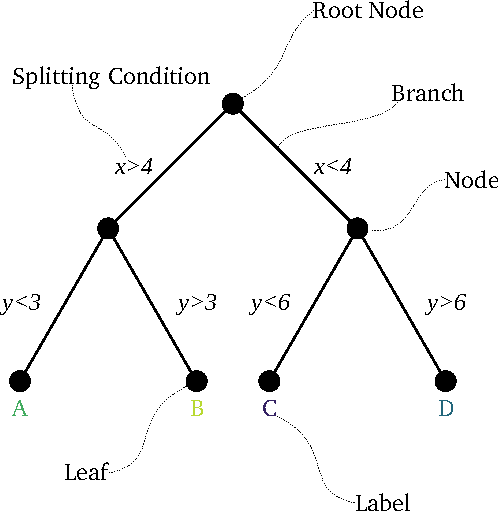
\includegraphics[width=\textwidth]{figures/decisiontree.pdf}
		\label{fig:decisiontreegrapha}
		\subcaption{}
	\end{subfigure}\noindent
	~
	\begin{subfigure}[c]{0.45\textwidth}
		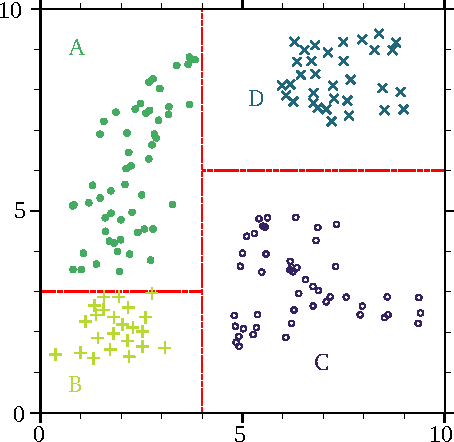
\includegraphics[width=\textwidth]{figures/decisiontreegraph.pdf}
		\label{fig:decisiontreegraphb}
		\subcaption{}
	\end{subfigure}
	\caption[Visual Explanation of Decision Trees]{(a) Example of a decision tree with the description of the individual elements; (b) Data that is classified based on the exemplary decision tree; A decision tree and the geometrical representation of the classification process is shown for a simple 2-D data set comprising four different classes with the labels A, B, C and D. The data virtually enters the decision tree at the root node. The splitting condition defines if the subsets get funnelled into the right or left branch. At the second nodes, the other splitting criteria are applied, and eventually, the data reaches the leaves where the labels are assigned.\cite{Forsyth2019}}
	\label{fig:decisiontreegraph}
\end{figure}\noindent
Three cardinal algorithmic questions arise from the described procedure: How to choose the feature on which to split the data? How to choose the splitting condition? And how to assign class labels to the leaves?\cite{Forsyth2019}\\
The simplest of these questions is the first one. The features of a decision tree are chosen at random. There are other options for generating a decision tree but the most common. Interestingly, carefully choosing the features taken into account by different nodes does not add great value to the classification process. \cite{Forsyth2019} However if $X$ contains many features that do not contribute to the classification problem (e.g., having a variance close or equal to zero), that approach can backfire. The probability that the decision tree chooses too many redundant features hinders its predictive capabilities.\cite{Forsyth2019}\\
The second question about the splitting condition can be solved by applying information theory. There are several methods to determine a splitting condition. The information gain method is described here as an example. First, the splitting conditions are determined during the training phase or fitting of a decision tree. During training, all true labels, $z$, of the data set, are known to the algorithm. Therefore a good heuristic is to gain as much information as possible for a given split. Information gain refers to the enrichment of datapoints with common labels within each subset. To obtain the entropy $H(D_{l})$ of the left subset $D_{l}$, the frequency of a class label $c$ within this subset is multiplied with its binary logarithm and then summed up over all different class labels. The frequency of $c$ within $D_{l}$ is calculated by dividing the number of corresponding labels $n(c;D_{l})$ by the total number of data points in $D_{l}$, $N(D_l)$. The entropy of the right subset after splitting is obtained accordingly.\cite{Forsyth2019}
\begin{align}\label{eq:entropy}
H(D_{l}) & = \sum_{c} \left[\frac{n(c;D_{l})}{N(D_{l})} \log _{2}\left( \frac{n(c;D_{l})}{N(D_{l})} \right)\right]
\end{align}\noindent
$H(D)$ corresponds to the number of bits necessary to classify a data point in the parent data set. Thus, $H(D_{l})$ and $H(D_\text{r})$ are the bits required to encode the labels within the left and right branch subsets. The information gain is defined as weighted entropies of the split subsets subtracted from the parent data set's entropy. Herein, the entropy of the split subsets $H(D_{l})$ is weighted by the probability to find items in the corresponding pool ($w_{l}$ or $w_\text{r}$).\cite{Forsyth2019}
\begin{align}\label{eq:weightentropy}
w_\text{r}  = \frac{N(D_\text{r})}{N(D)} \qquad \qquad &
w_{l} = \frac{N(D_{l})}{N(D)}
\end{align}\noindent
Finally, the information gain $I$ of a certain node is given by \fref{eq:infogain}.\cite{Forsyth2019}
\begin{align}\label{eq:infogain}
I & = H(D) - w_\text{r}\cdot H(D_\text{r}) - w_{l}\cdot H(D_{l})
\end{align}
In general, the greater the information gain, the better the split. From here, it is straightforward to obtain the optimal splitting condition. The inputs $X$ of the data set $D$ have a certain number of features $f$ (usually corresponding to columns) and datapoints $d$ (usually corresponding to rows). Within the assigned feature of the node $f$, there are $d$ data points which means there are $d-1$ possible splits that would change the composition of $D_{l}$ and $D_\text{r}$. Hence, the information gain is computed for every $d-1$ possible splits, and the threshold resulting in the best information gain is kept as a parameter for that node.\cite{Forsyth2019} The concept of splitting is visualized in \fref{fig:rfsplitting}.
\begin{figure}[H]
	\centering
	\includegraphics[width=0.8\textwidth]{figures/rfsplitting.pdf}
	\caption[Visualization of the Splitting Condition]{Visualization of the splitting condition. One feature of the data points is tested for optimal information gain. The two classes A and D are plotted along feature $f$, and the optimal split is marked in blue, whereas all other splits are denoted as red dotted lines.}
	\label{fig:rfsplitting}
\end{figure}\noindent
Eventually, the leaves are reached and assign labels to the data points in the final subsets. One leave will assign the majority label, present in the final subset during training. One decision tree is considered a very poor classifier. Many decision trees, on the other hand, can become very powerful. A \ac{rfc} comprises a large set of decision trees. A sample enters every pre-trained decision tree within the \ac{rfc}, and every decision tree computes a label. The simplest \ac{rfc} uses a majority vote to determine each label, i.e. the label most trees computed for that sample is assigned.\cite{Forsyth2019}\\
Apart from the splitting conditions, the feature selection and other parameters dictate a decision tree's behaviour and, therefore, of the \ac{rfc}. Those parameters are referred to as hyperparameters. These hyperparameters control how many trees are included in a \ac{rfc}, how deep the branches go, how many features they are allowed to use, to name a few.\cite{Pedregosa2012} As opposed to the splitting condition, which is chosen by mathematical optimization, the hyperparameters have to be entered by the operator.\cite{Forsyth2019}
%
%
\section{Cross Validation and Splitting}\label{sec:cv}
Usually, an advanced \ac{ml} model has enough parameters to fit a given data set optimally, therefore 'memorizing' the inputs and their corresponding labels. If a dataset used for training in its entirety was also used to test the resulting model, the model's performance would be near perfect. However, the
performance on unseen data would be inferior since the model would not abstract from the training dataset.\cite{Raschka2018}\\
Splitting the data and using one part for training and one part for performance estimation mitigates the selection bias. However, given the random splitting of the data, the model will not explore the complete data set, and the individual splits can have a biased label distribution. This bias would result in an underestimation of the performance. Both the issue of overfitting (or selection bias) and insufficient use of the data set can be circumvented by \ac{cv}.\cite{Forsyth2019}\\
During \ac{cv} the data set is split in $k$ subsets with equal sample count. These subsets are referred to as folds. Next, the model iterates through $k$ cycles of training and evaluation. In every cycle, another fold is used as a validation set, whilst the remaining $k-1$ folds are used for training. All evaluations are then averaged to yield a better estimate of the true model performance. This method of splitting the data set into $k$ folds and then cycling through each combination is called $k$-fold \ac{cv}\cite{Raschka2018} A visual representation is shown in \fref{fig:cv}.\\
\begin{figure}[H]
	\centering
	\includegraphics[width=\textwidth]{figures/cv_visualization.pdf}
	\caption[Visualization of \ac{cv}]{Visualization of \ac{cv}. The whole data set contains 83\% negative (green) data points and 17\% positive (purple) data points. It is split up into five equally large subsets of equal distributions of positive and negative samples. For 5-fold \ac{cv} the \ac{ml} model is trained five times. Each iteration uses another subset for validation (indicated by the lighter shade) whilst the others are used for training. The individual performances are averaged to yield a good estimate of the predictive power of the model.}
	\label{fig:cv}
\end{figure}
Selecting the hyperparameters is another caveat that results in performance overestimation. Hyperparameters were mentioned in \fref{sec:randomforestbackground} which are parameters specified by the user that dictate the model's architecture (i.e. the number of decision trees, branching depth, etc.). Those parameters are usually optimized by applying an automatic sampling of different values for each parameter. One possibility is to supply a value list for each hyperparameter which is called a parameter grid. The algorithm uses every combination of values consecutively to find the hyperparameters that perform best. Thus, the hyperparameter selection itself exploits information in the data. Otherwise, the hyperparameter variation would not impact the prediction performance. Therefore, optimizing the hyperparameters and using \ac{kfcv} on the \ac{rfc} parameter optimization only still results in exaggerated model performance. The application of \ac{kfcv} to the hyperparameter optimization as well as to the training of the \ac{rfc} solves this issue and is called nested \ac{kfcv}. The concept is shown in \fref{fig:nestedcv}.\cite{Raschka2018}
\begin{figure}[H]
	\centering
	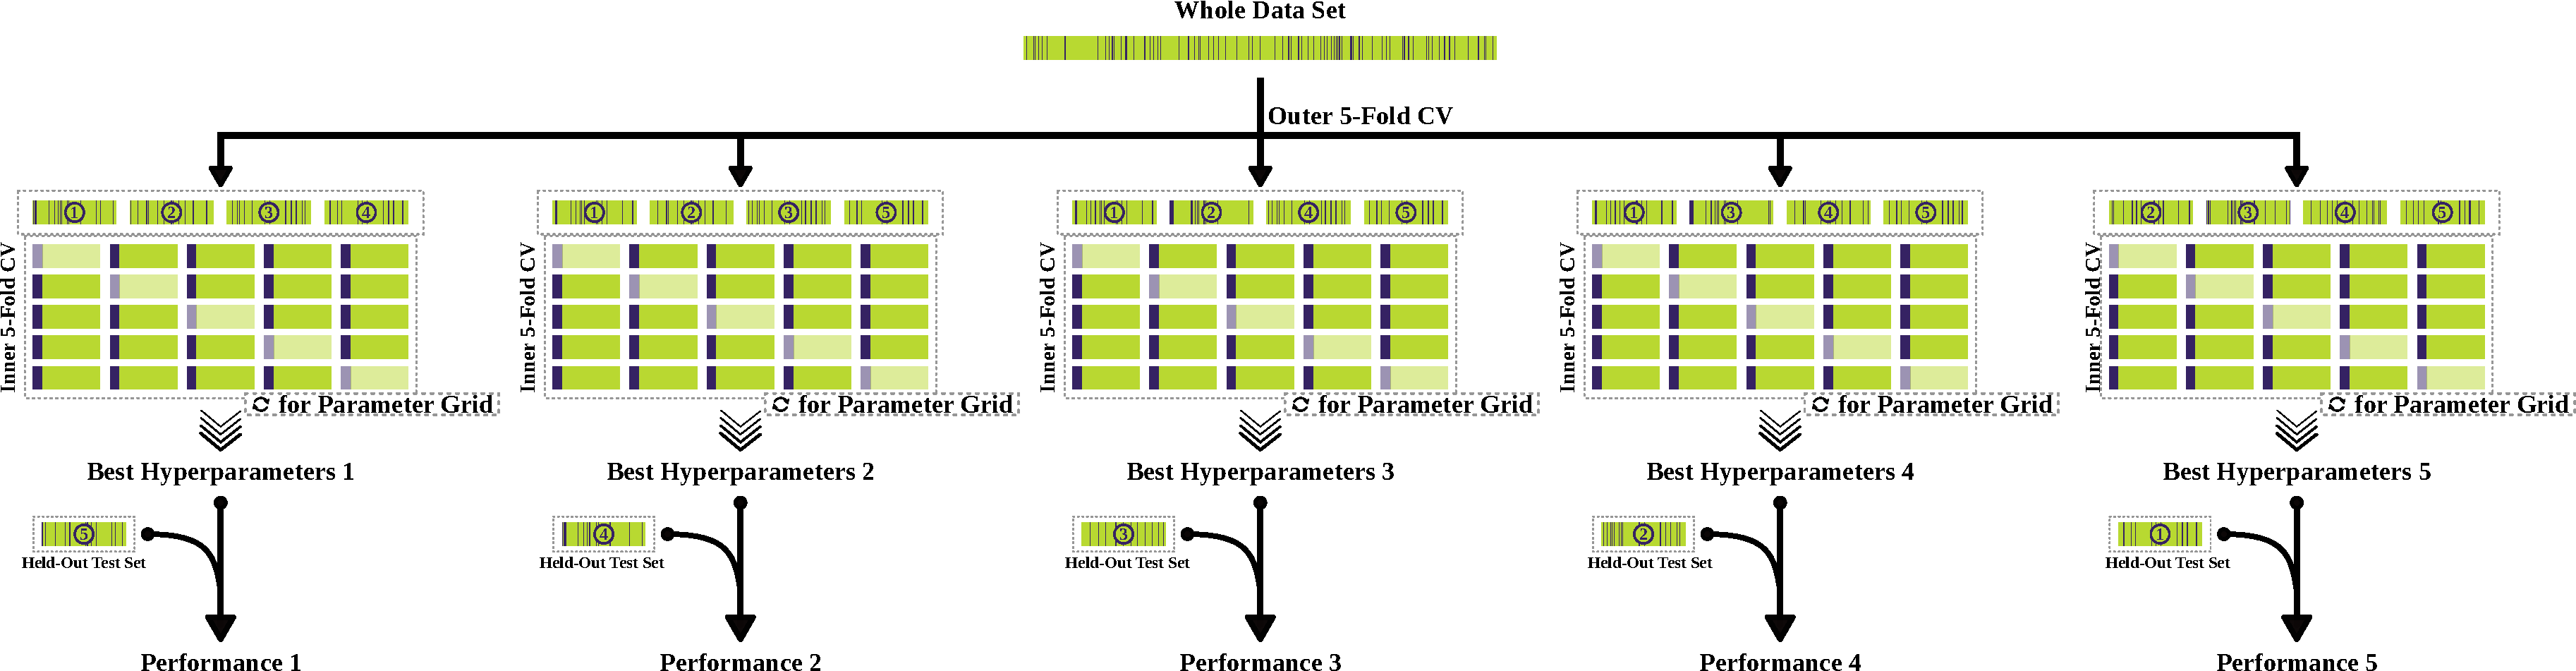
\includegraphics[width=\textwidth]{figures/nested_cv_visualization.pdf}
	\caption[Visualization of Nested \ac{cv}]{Visualization of nested \ac{cv}. The whole data set contains 83\% negative (green) and 17\% positive (purples) samples. The outer \ac{cv} splits the data into five subsets. Four of these subsets are used in the inner \ac{cv}. The other one will be used as a held-out test set for performance evaluation. The outer \ac{cv} results in five instances, each considering a different subset for evaluation. The inner \ac{cv} starts by splitting the outer training set into five subsets. Next, those subsets are used for training and evaluating all hyperparameter combinations supplied in the parameter grid. The best parameters are then tested to estimate the model performance.}
	\label{fig:nestedcv}
\end{figure}
The splitting strategy that is chosen should be as unbiased as possible to diminish performance overestimation. However, the distribution of labels within each fold should be comparable to avoid underestimation of the performance. In the worst case, one fold could contain all labels, which would lead to inferior prediction performance. The random-stratified-split-strategy splits the data set into randomly chosen subsets, each exhibiting an equal label distribution that counteracts pessimistic prediction performance.\cite{Kohavi1995}
%
%
\section{Performance Evaluation}\label{sec:perfeval}
There are several different metrics available for performance evaluation of an \ac{rfc}. Since the work presented here is concerned with a binary classification problem (i.e. only two labels are possible per sample), the descriptions below are only valid for binary classification. The most fundamental performance assessment of a classifier is given by the confusion matrix, which compares the predicted labels with the true labels. From the confusion matrix more applied metrics can be calculated, namely the \ac{tpr}, the \ac{tnr}, the \acl{ba}, the \ac{mcc} and many more. Furthermore, the \ac{roc} and \ac{auc} supply further information about the goodness of the fitted model.\cite{Fawcett2006}
%
\subsection{Confusion Matrix}\label{sec:confmatr}
A confusion matrix compares the predicted labels with the true labels of the classification problem. The confusion matrix is a quadratic matrix of the number of different classes (also referred to as the contingency table). For a binary classification problem, the confusion matrix is, therefore, a two by two matrix. The correctly identified instances are shown on the diagonal of the matrix, either referring to \ac{tp} or \ac{tn} instances. Off diagonal erroneously identified instances are presented, either \ac{fp} or \ac{fn} values. The general structure of a confusion matrix is shown in \fref{fig:confmat}.
\begin{figure}[H]
	\centering
	\begin{subfigure}[c]{0.35\textwidth}
		\centering
		\includegraphics[width=0.8\textwidth]{figures/confmatblank.pdf}
		\subcaption{Structure of a confusion matrix}
		\label{fig:confmat1}
	\end{subfigure}
	~~~~~~~~~~
	\begin{subfigure}[c]{0.35\textwidth}
		\centering
		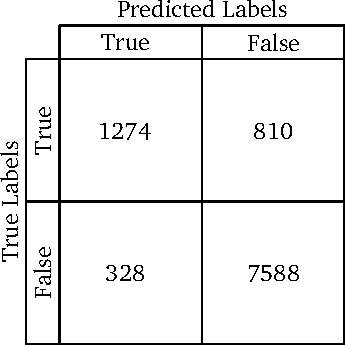
\includegraphics[width=0.8\textwidth]{figures/confmatexemp.pdf}
		\subcaption{Confusion matrix with exemplary values.}
		\label{fig:confmat2}
	\end{subfigure}
	\caption[Structure of a Confusion Matrix]{The general structure of a binary confusion matrix is shown on the left and on the right exemplary values are inserted in the respective fields.}
	\label{fig:confmat}
\end{figure}\noindent
\subsection{TPR, TNR, Balanced Accuracy and Matthews Correlation Coefficient}\label{sec:metrics}
From the confusion matrix several other metrics can be computed. For example the \ac{tpr} and \ac{tnr}, more widely known as the sensitivity and the specficity, aswell as the \ac{ba} and the \ac{mcc}. The \ac{tpr} describes the frequency of correctly positive-labelled samples whereas the \ac{fpr} depicts the frequency of incorrectly positive-labelled predictions.\cite{Fawcett2006}
\begin{align}\label{eq:tpr}
TPR & =\frac{TP}{TP+FN}
\\FPR & =\frac{FP}{TP+FN}
\end{align}
Analogously, the \ac{tnr} describes the frequency of the correctly negative-labeled samples within the predictions.\cite{Fawcett2006}
\begin{align}\label{eq:tnr}
TNR & = \frac{TN}{TN+FP}
\end{align}
The \acl{ba}, $BA$, is simply the average of the \ac{tpr} and the \ac{tnr}.\cite{Kelleher2015}
\begin{align}\label{eq:balacc}
BA & = \frac{TPR+TNR}{2}
\end{align}
$TPR$, $TNR$ and $BA$ can all adapt values between zero and one. One correponds to a perfect model. The \acl{mcc}, $MCC$, is a metric that scores high if the number of correctly predicted samples is significantly higher than the number of incorrectly assigned ones.\cite{Boughorbel2017}
\begin{align}\label{eq:mcc}
MCC & = \frac{TP\cdot TN - FP\cdot FN }{\sqrt{\left(TP+FP\right)\left(TP+FN\right)\left(TN+FP\right)\left(TN+FN\right)}}
\end{align}
The \ac{mcc} can score between -1 and 1 where 1 represents very good performance, 0 refers to a random model and -1 describes consistently false predictions.\cite{Boughorbel2017}
%
\subsection{ROC and AUC-ROC}\label{sec:rocauc}
\acp{rfc} assign discrete prediction labels $z$ to their input samples. However, as stated in \fref{sec:randomforestbackground}, a majority voting of the total number of trees is conducted. The majority voting can be interpreted as a probability $p$ for a certain class label by dividing the votes for a certain class label by the total number of votes. The resulting probability is between 0 and 1. A threshold $t$ can be applied that determines the label depending on the probability.
\begin{align}
z =  
\begin{cases}
0 & \text{if } p<t\\
1 & \text{if } p\geq t
\end{cases}
\end{align}
A majority voting refers to a threshold of \num{0.5}. However, the threshold can be varied from 0 to 1. For a zero threshold, all labels will be predicted as 'positive' (i.e. '1') since no label will have $p$ smaller than zero. For a threshold of one, all predictions will be 'negative'. Hence, for each threshold, a different confusion matrix is obtained and, therefore, a different \ac{tpr} and \ac{fpr}. For the \ac{roc} the \ac{tpr} is plotted on the y-axis and the \ac{fpr} is plotted on the x-axis. The threshold mentioned above is iterated from 0 to 1 to obtain all different confusion matrices from which the \ac{tpr} and \ac{fpr} are calculated. The \ac{auc} corresponds to the goodness of the model depicted by the corresponding \ac{roc}. An \ac{auc} of \num{1} is a perfect score since it corresponds to the aforementioned perfect \ac{roc}. The benefit of the \ac{roc} and \ac{auc} is that it contains more information than the other metrics and enable quick visual confirmation.\cite{Fawcett2006} In \fref{fig:roccurves} different \ac{roc} are shown that correspond to well or not so well-performing models.
\begin{figure}[H]
	\centering
	\includegraphics[width=0.7\textwidth]{figures/roccurves.pdf}
	\caption[Examples of ROC-Curves]{Examples of ROC-curves. The diagonal depicts a model that chooses labels randomly. If a curve is above the diagonal it predicts better than random, below indicates a bias towards the wrong label.}
	\label{fig:roccurves}
\end{figure}
%
%
\section{Feature Importance}\label{sec:featimport}
There are three methods of choice to measure feature importance that are used in this project: \ac{pca}, random forest feature importance and the \ac{mrmr}. \ac{pca} can be understood as a method of dimensionality reduction. The original data is mapped to a new coordinate system chosen by maximizing the variation in each dimension.\cite{Jolliffe2002} Therefore, the number of new axes, referred to as principal components, is the same as the original dimensionality. However, the first few principal components usually account for a large part of the variance within the -data set. In contrast, the lowest principal components account for no variance, which is referred to as noise in data science.\cite{Forsyth2019} Transforming the coordinate system also gives information about the contribution of each feature to the principal components, which can be used to infer feature importance for the original data set.\cite{Jolliffe2002}\\
Random forest feature importance can be either measured by \acl{gi} or by entropy (or information gain, see \fref{sec:randomforestbackground}). The gini impurity is defined as the product of probabilities to encounter positive samples, $p_1$ and negative samples $p_0$ respectively at a given node $k$.\cite{Zhang2012}
\begin{align}\label{eq:giniimpfornode}
G_k = 2p_1p_0
\end{align}
From \fref{eq:giniimpfornode} follows, that a small \acl{gi} refers to a very succesful split from the parent node with the index $k-1$. If both descendant nodes contain one label only, the parent node has achieved the best split possible. The feature importance for a single decision tree $I^{(f)}_\text{d}$ is therefore defined as the sum of reductions in \acl{gi} from every parent node $k$ that uses feature $f$ in its splitting condition to its descendants $k+1$.\cite{Zhang2012}
\begin{align}\label{eq:giniimptree}
I^{(f)}_\text{d} & = \sum_{k} G_{k}^{(f)} - G_{k+1}
\end{align}
Notice, that $G_{k+1}$ comprises the contribution of the left and right descendant nodes. The overall feature importance of feature $f$ is calculated as the the average of tree-wise feature importances.\cite{Zhang2012}
\begin{align}\label{eq:giniimpforest}
I^{(f)} & = \frac{1}{N_d}\sum_{d}I^{(f)}_\text{d}
\end{align}
$N_d$ is the number of trees in the \ac{rfc}. Since the splitting at node $k$ always incorporates the information from prior nodes, this method of feature importance accounts for non-linear feature interaction. One shortcoming of this method is that strongly correlated features tend to share their importance, which results in two difficulties. Firstly, critical features are scored lower since the importance measure is split within highly correlated feature clusters. Secondly, the final selection will contain many features that belong to the same highly correlated cluster. Adding many features that contain similar information has no beneficial effect on the model and fosters biased predictions based on a few clusters' information. To overcome these two problems, hierarchical clustering can be performed on the features beforehand, and from every cluster, only one feature is picked for further feature engineering.\\
\ac{mrmr} is a feature selection algorithm that was proposed by Peng \textit{et al.}.\cite{Peng2005}. It utilizes mutual information between features to calculate their redundancy and mutual information between features and each class label to calculate maximum relevance to the categorization problem. The algorithm then optimizes the subtraction of the features redundancy and the feature relevance to obtain a scoring for each feature. \ac{mrmr} was found to be very suitable for data sets with more than 1000 numerical features.\cite{Peng2005}
%
%
\section{Gene Ontology Terms}\label{sec:geneontologyBackground}
% intro
The \ac{go} terms are keywords assigned to genes and their products by the Gene Ontology Consortium. The vocabulary is structured, precisely defined and controlled.\cite{Ashburner2000}\\
% biological processes
Three main categories are distinguished within \ac{go} terms: biological processes, molecular function and cellular component. A biological process is defined as a process that involves a chemical or physical transformation. Thus, something enters a process and is released as something else. High-level examples include \ac{go} terms like 'cell growth and maintenance'. A more specific example would be 'cAMP biosynthesis'.\cite{Ashburner2000}\\
% molecular function
Molecular function refers to the biochemical activities of a gene product. That corresponds to chemical reactions, binding mechanisms and transport mechanisms, to name a few. The molecular function does not specify where or when it happens, only that the gene product holds the potential to execute this function. High-level \ac{go} terms are 'enzyme', 'ligand' and low-level terms are 'adenylate cyclase' and 'Toll receptor ligand'.\cite{Ashburner2000}\\
% cellular component
The cellular component places a specific gene product within the cell. This placement does not necessarily correspond to a localized organelle. For example, 'proteome' is an adequate \ac{go} term within the cellular component. Other terms like 'Golgi apparatus' or 'nuclear memrane' refer to cellular components though.\cite{Ashburner2000}
% hierarchy
Terms within \ac{go} can be connected hierarchically. A specific molecular function like 'oxidoreductase activity' is a descendant from 'catalytic activity', for example. The three main categories can also be linked by logical operators, which produces hierarchical networks containing abundant information about a given gene product.\cite{Ashburner2000} Three exemplary hierarchical trees can be seen in \fref{fig:gotermtree}.\\
% when is a term included to \ac{go}?
\ac{go} database includes information about a gene product if published experiments are available or if information can be inferred from sequence homology, which is mostly applied to less studied organisms. The information gained from these sources must fulfil evidence requirements set by Evidence and Conclusion Ontology (ECO).\cite{Ashburner2000,Carbon2020}
\begin{figure}[H]
	\centering
	\includegraphics[width=0.95\textwidth]{figures/goterms.pdf}
	\caption[Examples of \ac{go} Term Hierarchies]{Examples of \ac{go} term hierarchies. (a) is an example of a biological process; (b) presents a molecular function \ac{go} tree; (c) is an example of a cellular component; (d) is a tree that is a mix of biological process and molecular function; (d) is an exhaustive legend defining colours as well as possible relationships.}
	\label{fig:gotermtree}
\end{figure}